\section{Exceptions}

\begin{multicols*}{2}
Behandelt unerwartete Programmzustände oder Ausnahmeverhalten zur Laufzeit.
\subsection{Best practices}
\begin{itemize}
    \item Exception sind Ausnahmen
    \item Wenn möglich Vorbedingungen prüfen um Exceptions zu vermeiden
    \item Exceptions sind Fehlercodes vorzuziehen
    \item Konkrete Fehlerbeschreibung 
    \begin{itemize}
        \item Möglichst konkrete Exception-Klassen verwenden
        \item Möglichst detaillierte Beschreibung des Fehlers
        \item Aber NIE über Web-Schnittstelle übermitteln (offenbart Internas und erhöht Verletzbarkeit des Systems)
    \end{itemize}
    \item Aufräumen bei Exceptions (Sockets, File Handles, offene Transaktionen, etc.)
\end{itemize}

\subsection{Schlüsselwörter}
\begin{lstlisting}
FileStream s = null; 
try
{
    s = new(@"C:\Temp\Test.txt", FileMode.Open);
    /* ... */
}
catch (FileNotFoundException e) {
    Console.WriteLine("{0} not found", e.FileName);
}
catch (IOException)
{
    Console.WriteLine("IO exception occurred");
}
catch
{
    Console.WriteLine("Unknown error occurred");
}
finally 
{
    if (s != null) s.Close();
}
\end{lstlisting}
\subsubsection{try}
Anweisungsblock welcher potenziell eine Ausnahme verursacht.
\subsubsection{catch}
\begin{itemize}
    \item Anweisungsblock der eine spezielle Ausnahme behandelt.
    \item catch-Block wird sequenziell gesucht
    \item Es wird pro Exception nur ein catch-Block ausgeführt
    \item Exception-Name darf entfallen falls nicht verwendet
    \item Exception-Typ muss nicht angegeben werden, es wird System.Exception angenommen
    \item Exception-Typ muss von System.Exception abgeleitet sein
\end{itemize}
\fat{Bedingter Catch:}
\begin{lstlisting}
try { /* ... */ }
catch (Exception e) when (DateTime.Now.Hour < 18) 
{
/* ... */
}
catch (Exception e) when (DateTime.Now.Hour >= 18)
{
    /* ... */
}
\end{lstlisting}
\subsubsection{finally}
Anweisungsblock, der nach einem try, sowie auch nach einem catch-Block garantiert einmal ausgeführt wird.
\subsubsection{throw}
Statement löst eine beliebige Exception aus
\begin{lstlisting}
throw new Exception("An error occured");

//Neuen Stack Trace beginnen mit e
catch (Exception e) 
{
    throw e; 
}

//Rethrowing: Stack Trace bleibt erhalten
catch (Exception e) 
{
    throw; 
}
\end{lstlisting}

\subsection*{System.Exception}
\begin{lstlisting}
public class Exception : ISerializable, _Exception
{
    public Exception();
    public Exception(string message);
    public Exception(string message, Exception innerException);
    //Verschachtelte Exception
    public Exception InnerException { get; } 
    //Fehlermeldung als String
    public virtual string Message { get; } 
    //Name des Objekts, welches den Fehler verursarchte
    public virtual string Source { get; set; } 
    //Methodenaufrufkette als String
    public virtual string StackTrace { get; } 
    //Ausgeführter Code-Teil der Fehler verursacht
    public MethodBase TargetSite { get; }
    public override string ToString();

    /* ... */
}
\end{lstlisting}
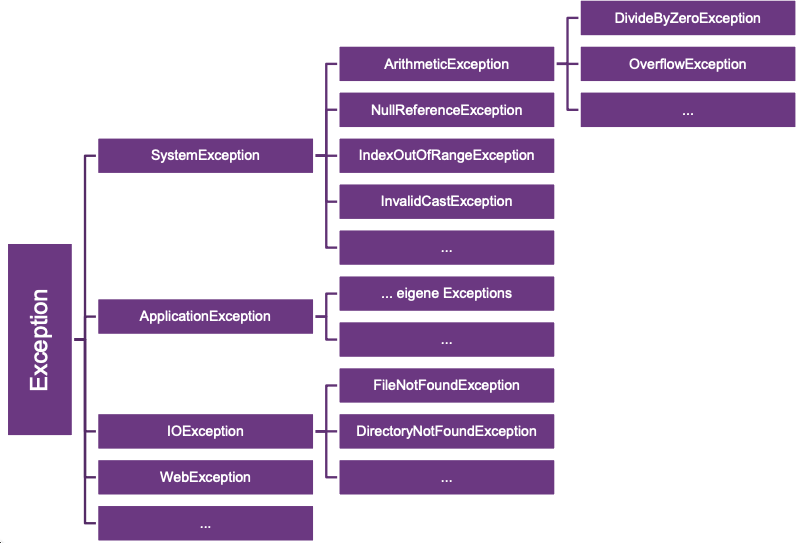
\includegraphics[width=\columnwidth]{exceptions}
\end{multicols*}